\documentclass[12pt]{article}

\usepackage{amsmath, graphicx}
\usepackage[margin=1in]{geometry}
\usepackage[font=footnotesize]{caption}
\usepackage[backend=bibtex]{biblatex}
\addbibresource{cs221proj.bib}
\usepackage[table,xcdraw]{xcolor}

\DeclareMathOperator*{\argmin}{arg\,min}
\DeclareMathOperator*{\argmax}{arg\,max}


\begin{document}
\nocite{*}

\title{Super Mario Bros with Deep Reinforcement Learning}

\author{
  Matthew Chen\\
  \small \vspace{-2mm} Department of Computer Science\\
  \small \vspace{-2mm} Stanford University\\
  \small mcc17@stanford.edu
  \and
  Isabel Bush\\
  \small \vspace{-2mm} Department of Computer Science\\
  \small \vspace{-2mm} Stanford University\\
  \small ibush@stanford.edu
}
\date{}
\maketitle

\begin{abstract}
We implement several reinforcement learning models to learn the optimal actions for a variant of the classic Super Mario Bros game. The game is challenging from an AI standpoint as the environment is stochastic, and the state space is large. Our algorithms use Q-learning with differing Q-function approximations including a linear and neural network approach. We test the effectiveness of the various approximations relative to their performance and runtime. We find that the neural network approximation performs best on our baseline task as well as across varying levels of difficulty.

\end{abstract}

\section{Related Work}

The Super Mario Bros competition started in 2009 as a way to benchmark AI algorithms on the task of creating an effective controller for the game \cite{togelius20102009}. In the first iteration, the best performing agents were ones based on open-loop path planning algorithms such A*. The most successful of these algorithms built an extensive internal model of the game to find optimal paths to the end goal. The best submissions that involved some form of learning for the follow-up competition were based off of a combination of search and evolutionary algorithms \cite{karakovskiy2012mario}.

Outside of the official competition there have been several attempts at using reinforcement for the simulation, such as Q-learning in \cite{liao2012cs229}. This implementation involves hand crafted features and uses a simple lookup as the Q-function approximation. To create a controller that can instead translate the raw input from the game to optimal actions, we draw inspiration from recent deep learning approaches applied in \cite{mnih2013playing}. In this study, researchers applied a convolutional neural network to map raw pixel values to actions for several Atari games and were able achieve super-human performance on several of the games they tested. In this paper we experiment with this approach to determine if a similar neural network can achieve high performance in the Mario game, which appears to be a more complex learning task.

\section{Models}

\begin{figure}[h]
\centering
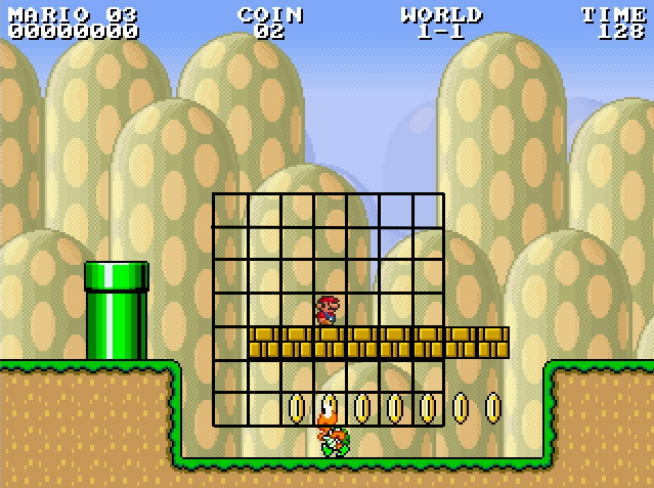
\includegraphics[scale=0.5]{imgs/mario_grid}
\caption{A component of the game state is a small grid centered around Mario indicating objects nearby. In the actual simulation, the grid is 22 x 22 cells, where each cell is the size of a single block \cite{karakovskiy2012mario}.}
\label{mario_grid}
\end{figure}

We choose the Q-Learning algorithm as our approach to this problem as it enables us to learn a controller without creating a model for the game or having a known reward function. Our approach experiments with different Q-function approximations such as identity, linear, and neural network. Additionally we employ an epsilon greedy strategy to ensure adequate exploration of the state space by taking a random action with probability 1 - $\epsilon$. The update rule and optimal action choice are as follows, where R is the reward for taking action a at state s and ending in state s', and $\alpha$ and $\gamma$ are the learning rate and discount factor, respectively.

\begin{align*}
Q(s,a) &\leftarrow Q(s,a) + \alpha (R + \gamma \max_{a' \in A} Q(s',a') - Q(s,a))\\
a^* &= \argmax_{a \in A} Q(s,a)
\end{align*}

Our state is defined as a vector of all observed attributes of the game. This can be divided into two components. In the first component are meta data features which include distance to the finish, time left, and Mario state (small, large, fireball power). These features describe the progression of the game. The second component is a 22 x 22 grid which is provided by the simulator at each time step, as shown in Figure \ref{mario_grid}. The grid can be thought of as a low detail/resolution view of the game. The entire grid is centered around Mario and each cell corresponds to objects in that relative position to Mario (blocks, mushrooms, monsters, gap, etc). We flatten this grid to get the underlying features.

Actions correspond to combinations of the original buttons which could be pressed for the player to interact with the game. The game uses a six element vector corresponding to the set of six buttons which can be toggled on and off during a given time-step (directional move, jump, and fireball). The up button has no affect and the down button is rarely used, so we removed these buttons to speed computation. Since combinations of buttons are possible, we have defined our set of possible actions as all binary combinations of the four remaining buttons leading to $2^4 = 16$ distinct actions.

The reward at each time-step is calculated as the change in fitness score over that time-step due to the action taken at the previous state. The fitness score is provided by the game and takes into account distance passed and coins collected.

\subsection{Identity Function}

Our first learning agent maps the full state representation vector to the best action to take from that state. Since the state space is very large (the state vector has length $733$, which yields upwards of $2^{733}$ distinct states) and many states are unlikely to be seen (creating a sparse feature vector), we stored the state-action mapping in a hashmap to allow for quick access and efficient space usage. This was the strategy deployed by \cite{liao2012cs229}, except their representation of state required high-level hand-crafted features while our representation uses low-level game features. Below we specify the Q-function and corresponding basis function which transforms a state action pair to the given state vector representation.

\begin{align*}
Q(s,a) &= Lookup(\beta(s,a))\\
\beta(s,a)_{i*j} &= 1\{ S_i = s \} * 1\{ A_j = a \}
\end{align*}

\subsection{Linear Approximation}

Our linear agent uses the same low-level game features, but fits a linear model to estimate the value function. This model approximates the Q-function by taking a dot product between a vector of learned weights and the input features. The feature vector consists of indicator values for each element of the state vector and every possible action. This yields a feature vector of length $|stateVector| * |Actions| = 733 * 16 = 11,728$. While still large, this is much less than the identity feature vector and can easily fit in memory. And more importantly, this allows the agent to generalize to unseen states and learn more quickly. The weight vector $\theta$ is learned using the Q-function below.

\begin{align*}
Q(s,a) &= \theta^T \beta(s,a)\\
\beta(s,a)_{i*j} &= 1\{ S_i = s \} * 1\{ A_j = a \}
\end{align*}

\subsection{Neural Network}

Our neural network implementation has even fewer input features than the linear agent. Since state/action interactions can be exposed by the network, the input feature vector can be simplified to the state vector and an indicator for the action chosen. The features are fed through two fully-connected layers, with associated rectified linear layers, to the final fully-connected output layer which provides an estimate for the Q-function.

\begin{align*}
Q(s,a) &= ForwardPass(\theta, \beta(s, a))\\
\beta(s,a)_{i} &= 1 \{ S_i = s \}\\
\beta(s,a)_{|S| + j} &= 1 \{ A_j = a \}
\end{align*}

Additionally, we experiment with using a playback memory as defined in \cite{mnih2013playing}. We store the previous N observations from the game. We then sample from these observations during a single update to perform mini-batch gradient descent. This method is used to help mitigate the problem of correlated features from time windows and aid in the convergence of the weights.

\section{Results}

\subsection{Method Comparison}

\begin{figure}
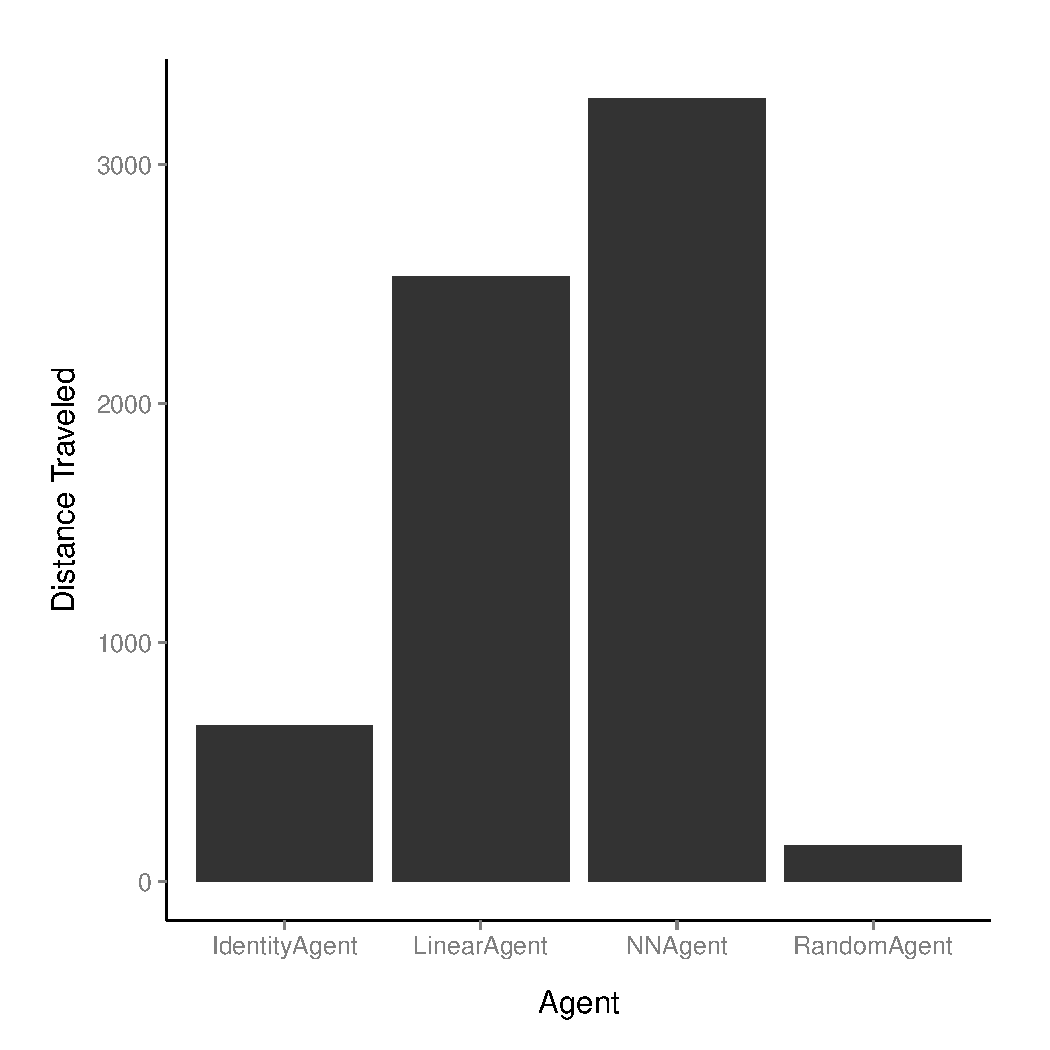
\includegraphics[scale=0.5]{imgs/dist_bar.pdf}
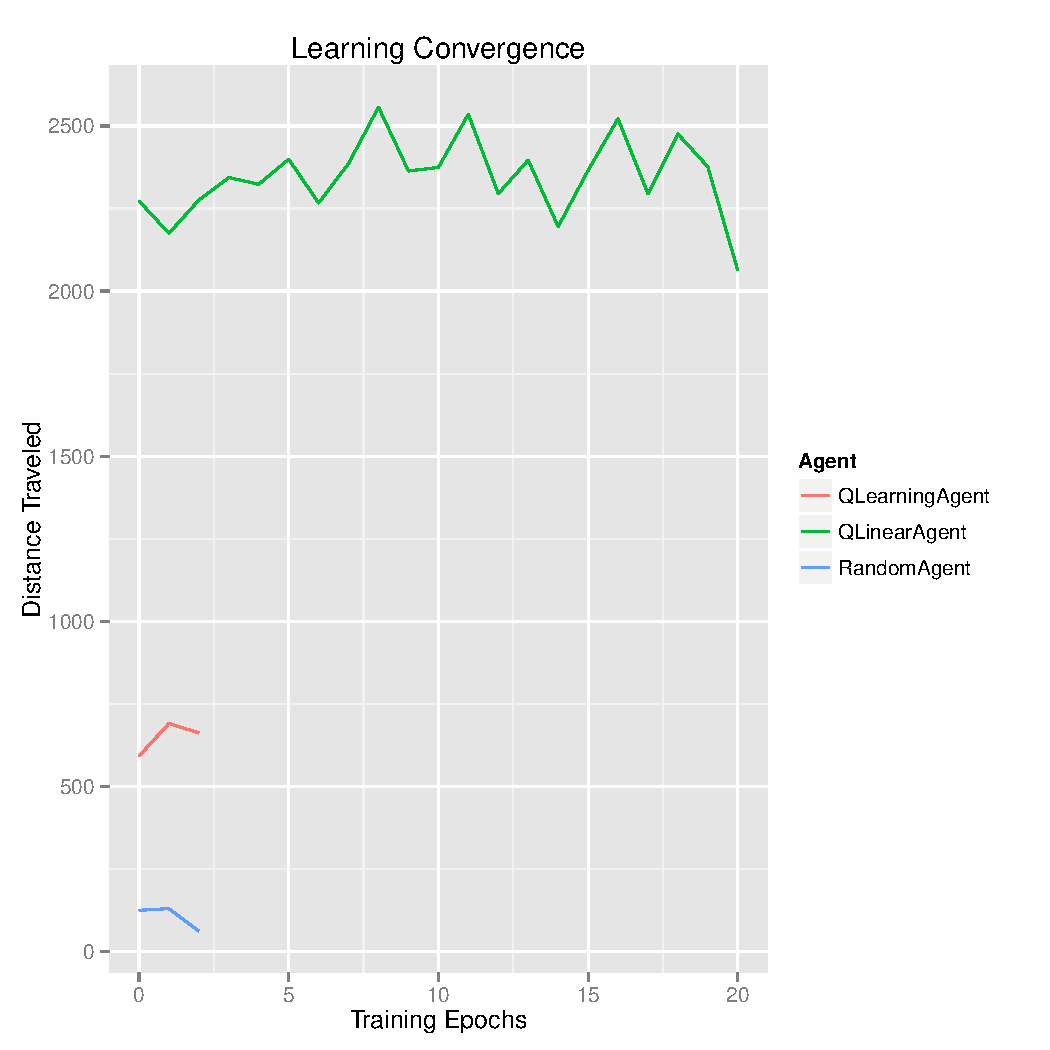
\includegraphics[scale=0.5]{imgs/dist_line.pdf}
\caption{Learning statistics showing comparison between different agents by mean progress before end of game}
\label{agent_comp}
\end{figure}

Our results comparing the different methods are shown in Figure \ref{agent_comp}. The average distance travelled can be seen in the left graph and the distance travelled over the trials can be seen in the right graph, showing learning convergence. Here we use the distance travelled toward the goal within a single game to measure performance. For this particular level, the length of the goal is 4096, which serves as an upper bound for any individual observation. We can see that all agents perform significantly better than our baseline random agent. 

The identity agent was able to run for about 200 trials before running out of memory (where each trial is a full game and consists of about 1000 time-steps). At the start of learning, Mario jumps around aimlessly performing random actions. By the end of the 200 learning trials, the agent has learned to move forward from some states and thus makes progress. However, since there is no generalization, the agent still performs random actions from many states and the game usually ends due to time-out. 

Due to generalization of state features, the linear agent learns much faster than the identity agent, as can be seen by the higher distance travelled even during the first few training epochs. The rate is faster despite a much lower learning rate, which was needed to keep the weights from diverging. The linear agent is able to progress farther on average than the identity agent (generalizing the desire to move forward to many different states) and thus usually completes the level or dies from a monster rather than hitting the timeout. 

The performance of our neural network agent starts at the level of the linear agent in the first few epochs. However after this point it reaches another plateau at a higher average distance travelled. We can also observe that the variability of results decreases in the later epochs which is likely due to the annealed learning rate leading to a convergence of the Q-function approximation.

\subsection{Runtime Analysis}

\begin{figure}
\begin{minipage}{0.5\textwidth}
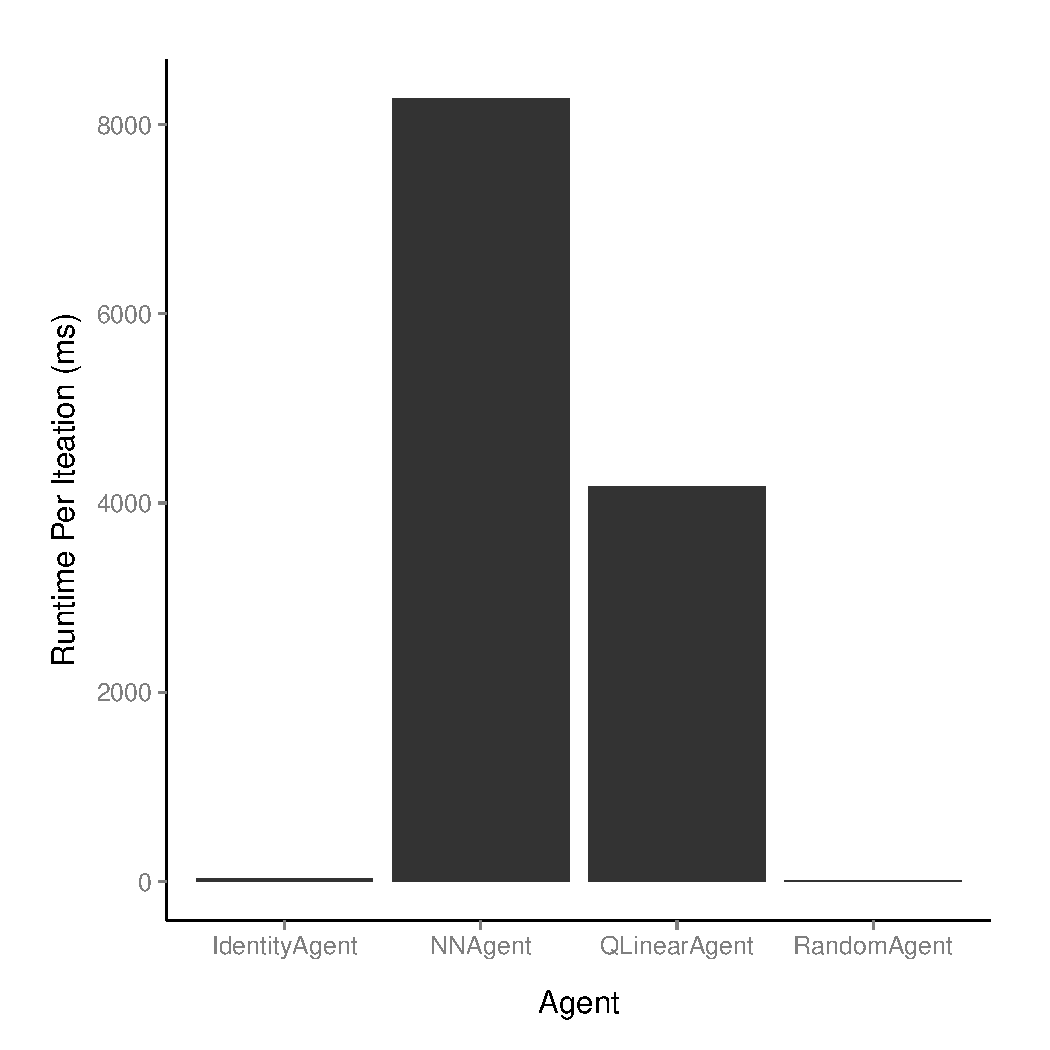
\includegraphics[scale=0.5]{imgs/runtime_bar.pdf}
\caption{Mean runtime per step by method}
\label{runtime_bar}
\end{minipage}
\begin{minipage}{0.5\textwidth}
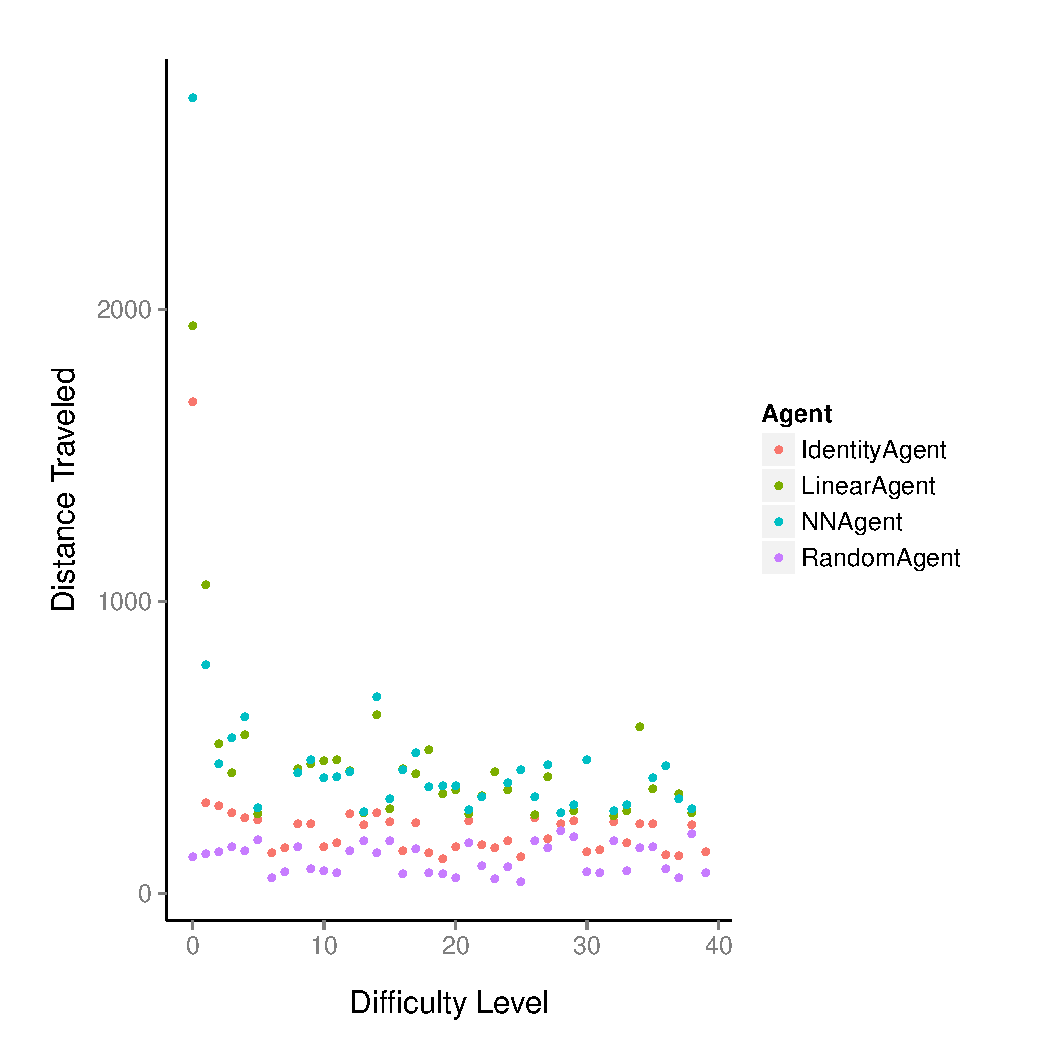
\includegraphics[scale=0.5]{imgs/dist_levels.pdf}
\caption{Comparison between different agents by mean progress in each level}
\label{scatter_levels}
\end{minipage}
\end{figure}



We plot the runtime per step in Figure \ref{runtime_bar}. A step involves the agent updating parameters as well as choosing an action. We can see that random agent and identity agent are very fast in choosing an action, but as we saw previously, these agents have the worst performance. This is intuitive as the random agent does not have parameters to update and simply uses a random number generator. While the identity agent does have an update step it only does add and lookup operations.

Conversely, both the neural network agent and the linear agent take a non-trivial amount of time to update. Both update and action evaluation steps for these agents require matrix multiplications. These networks however performed the best. As we can see there is a trade-off between agent speed and performance. Still, these update times are well within the 42ms of available time between frames at the standard simulation speed of 24 fps.

\subsection{Parameter Tuning}

To tune hyperparameters for our agents, we implemented scripts to vary each of the hyperparameters and record the average distance travelled when trained using these values. 

We tested with varying static epsilon-greedy values as well as decreasing epsilon-greedy values. We found that the identity agent performs similarly with static and decreasing epsilon-greedy values. This is likely because it must choose a random action for any unseen states, regardless of the epsilon-greedy parameter (a random action is chosen even if the policy is to be greedy). For the linear and neural network agents, a decreasing epsilon-greedy value that begins at 1 and decreases by $\sqrt{updates / 10000}$ every 10,000 time-steps was found to perform the best. This allows these agents to explore the state-space at the beginning, but use the optimal policy as learning progresses and during analysis.

For the neural network we also tuned the size of hidden states. We found the distance travelled improved as the number of hidden states increased to about 50, but remained relatively constant after that. Since the computation time increases exponentially as the hidden state size increases, we set these values to 50. The replay memory also improved results between a size of 1 (no replay) and 100, but results are fairly steady when increased further. Thus a replay size of 100 could minimize the memory usage.

\subsection{Comparison to Previous Methods}


\begin{table}[]
\centering
\label{my-label}
\begin{tabular}{|l|l|l|ll}
\cline{1-3}
\textbf{Competitor}                                        & \textbf{Approach}                        & \textbf{Distance}                                &  &  \\ \cline{1-3}
Robin Baumgarten                                        & A*                                                & 46565                                                &  &  \\ \cline{1-3}
Peter Lawford                                                & A*                                                & 46565                                                &  &  \\ \cline{1-3}
Andy Sloane                                                  & A*                                                & 44736                                                &  &  \\ \cline{1-3}
Trond Ellingsen                                              & RB                                                & 20599                                                &  &  \\ \cline{1-3}
Sergio Lopez                                                & RB                                               & 18240                                                &  &  \\ \cline{1-3}
Spencer Schumann                                      & RB                                                & 17011                                                &  &  \\ \cline{1-3}
\cellcolor[HTML]{C0C0C0}{\color[HTML]{333333} NN Agent} & \cellcolor[HTML]{C0C0C0}{\color[HTML]{333333} RL, NN} & \cellcolor[HTML]{C0C0C0}{\color[HTML]{333333} 15998} &  &  \\ \cline{1-3}
\cellcolor[HTML]{C0C0C0}{\color[HTML]{333333} Linear Agent} & \cellcolor[HTML]{C0C0C0}{\color[HTML]{333333} RL} & \cellcolor[HTML]{C0C0C0}{\color[HTML]{333333} 14823} &  &  \\ \cline{1-3}
Matthew Erickson                                         & GP                                                & 12676                                                &  &  \\ \cline{1-3}
Douglas Hawkins                                          & GP                                               & 12407                                                &  &  \\ \cline{1-3}
Sergey Polikarpov                                        & NN                                                & 12203                                                &  &  \\ \cline{1-3}
Mario Perez                                                & SM                                               & 12060                                                &  &  \\ \cline{1-3}
\cellcolor[HTML]{C0C0C0}{\color[HTML]{333333} Identity Agent} & \cellcolor[HTML]{C0C0C0}{\color[HTML]{333333} RL} & \cellcolor[HTML]{C0C0C0}{\color[HTML]{333333} 9624} &  &  \\ \cline{1-3}
Alexandru Paler                                         & NN, A*                                          & 7359                                                &  &  \\ \cline{1-3}
Michael Tulacek                                        & SM                                               & 6572                                                &  &  \\ \cline{1-3}
Rafael Oliveira                                          & RB                                                & 6314                                                &  &  \\ \cline{1-3}
Glenn Hartmann                                       & RB                                                & 1060                                                &  &  \\ \cline{1-3}
\end{tabular}
\caption{Distance travelled by our Q-Learning agents compared with 2009 Mario Competition results from \cite{karakovskiy2012mario}. Approaches are A*, rule-based (RB), reinforcement learning (RL), neural network (NN), genetic programming (GP), and state machine (SM).}
\label{table_levels}
\end{table}

To compare our agents to previous Mario controllers, we ran our agents through 40 levels of increasing difficulty, as was done in the Mario competition \cite{karakovskiy2012mario}. We trained our agents for 2000 trials on each level, then compared the averages of the last 50 trials for each agent. The averages can be seen in Figure \ref{scatter_levels} and the sum across all levels compared against competition controllers is shown in Table \ref{table_levels}. 

The success of the agents clearly drops quickly as the difficulties increase, however the more sophisticated models still outperform the simpler ones. Comparing the sum of scores across all levels to the competition results, we find that our linear and neural network reinforcement learning agents outperform all genetic programming, neural network, and state-machine models from the competition, but fall short of the results of A* and some rule-based agents.

\section{Discussion}

We started our Q-learning agent with the identity agent which attempts to map low-level features to a value. While this is a simple model that is able to learn some of the game's objectives, it has a few shortcomings. First, since this simple Q-learning model maps directly from states to actions, no generalization may be made to unseen states. The best action to take from each state must be learned independently, and the agent will choose a random action for any new state (even if very similar to a past state). This makes learning slow and inefficient. Second, an implementation shortcoming of this model is that the large feature vector consisting of all possible states can overflow memory. This limits the number of learning trials that may be run as the memory-usage grows with each new state.

Next our linear agent attempted to solve these issues by having a linear function approximation for the Q-value. This method allowed us to store information about states in a fixed size vector. It also allowed for generalization as unseen states were given a score with some basis in experience. The linear agent performed very well relative to our baseline method and the identity agent for these reasons. The limitation for the linear agent is the linear assumption in the function approximation is likely too constraining to be a good estimate of the true Q-value function. This is due to the fact that the features, such as the grid input, are not independent of one another.

Our Q-agent with a neural network function approximation aimed to address some of the limitations of the linear function approximation. The use of several hidden layers with rectified linear unit non-linearities allows us to approximate more complex functions. Additionally, in order to help the convergence of the weights, we implemented replay memory to store previous observations and randomly sample a subset for each update. This lead to an agent that performed better than our linear agent. However the performance improvements come at a cost in terms of runtime as it takes  longer to compute each move relative to our other approaches.

Although none of our agents were able to outperform the top agents from the Mario AI competition, our linear and neural network agents were only topped by A* and rule-based controllers, which require extensive knowledge of the game setup and rules. Considering that our agents learned all of this game information from only the raw input provided by the simulation, we believe this shows great promise for using reinforcement learning on the Mario game. The advantage of these learning agents, as compared to the search and rule-based agents, is that if presented with a very different environment (with new rules, obstacles, and rewards), these agents would adapt to the new environment without any model modifications.


\printbibliography

\end{document}